\documentclass{standalone}
\ifx\HCode\UnDef\else\def\pgfsysdriver{pgfsys-tex4ht.def}\fi
\usepackage{tikz}
\usepackage{color}
\usepackage{siunitx}
\usetikzlibrary{arrows,shapes}
\begin{document}
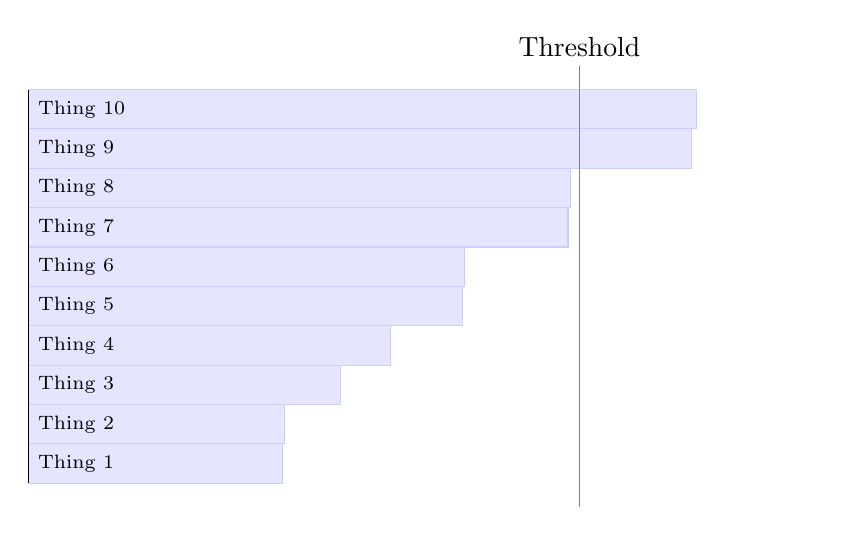
\begin{tikzpicture}
\begin{scope}[]
\clip (0.0,0.0) rectangle (10.0,5.0);
\begin{scope}[shift={(0.0,0.0)}]
\pgfsetxvec{\pgfpoint{0.028571429cm}{0cm}}
\pgfsetyvec{\pgfpoint{0cm}{0.5cm}}
\begin{scope}[shift={(0.0,0.0)}]
\begin{scope}[draw=blue!20,fill=blue!10]
\pgfpathmoveto{ \pgfpointxy {0.0} {10.0}}
\pgfpathlineto{ \pgfpointxy {297.0} {10.0}}
\pgfpathlineto{ \pgfpointxy {297.0} {9.0}}
\pgfpathlineto{ \pgfpointxy {295.0} {9.0}}
\pgfpathlineto{ \pgfpointxy {295.0} {8.0}}
\pgfpathlineto{ \pgfpointxy {241.0} {8.0}}
\pgfpathlineto{ \pgfpointxy {241.0} {7.0}}
\pgfpathlineto{ \pgfpointxy {240.0} {7.0}}
\pgfpathlineto{ \pgfpointxy {240.0} {6.0}}
\pgfpathlineto{ \pgfpointxy {194.0} {6.0}}
\pgfpathlineto{ \pgfpointxy {194.0} {5.0}}
\pgfpathlineto{ \pgfpointxy {193.0} {5.0}}
\pgfpathlineto{ \pgfpointxy {193.0} {4.0}}
\pgfpathlineto{ \pgfpointxy {161.0} {4.0}}
\pgfpathlineto{ \pgfpointxy {161.0} {3.0}}
\pgfpathlineto{ \pgfpointxy {139.0} {3.0}}
\pgfpathlineto{ \pgfpointxy {139.0} {2.0}}
\pgfpathlineto{ \pgfpointxy {114.0} {2.0}}
\pgfpathlineto{ \pgfpointxy {114.0} {1.0}}
\pgfpathlineto{ \pgfpointxy {113.0} {1.0}}
\pgfpathlineto{ \pgfpointxy {113.0} {0.0}}
\pgfpathlineto{ \pgfpointxy {0.0} {0.0}}
\pgfusepath{ stroke, fill, }
\end{scope}
\begin{scope}[draw=blue!20,fill=blue!10]
\pgfpathmoveto{ \pgfpointxy {0.0} {10.0}}
\pgfpathlineto{ \pgfpointxy {0.0} {10.0}}
\pgfusepath{ stroke, }
\end{scope}
\begin{scope}[draw=blue!20,fill=blue!10]
\pgfpathmoveto{ \pgfpointxy {0.0} {10.0}}
\pgfpathlineto{ \pgfpointxy {297.0} {10.0}}
\pgfusepath{ stroke, }
\end{scope}
\begin{scope}[draw=blue!20,fill=blue!10]
\pgfpathmoveto{ \pgfpointxy {0.0} {9.0}}
\pgfpathlineto{ \pgfpointxy {297.0} {9.0}}
\pgfusepath{ stroke, }
\end{scope}
\begin{scope}[draw=blue!20,fill=blue!10]
\pgfpathmoveto{ \pgfpointxy {0.0} {9.0}}
\pgfpathlineto{ \pgfpointxy {295.0} {9.0}}
\pgfusepath{ stroke, }
\end{scope}
\begin{scope}[draw=blue!20,fill=blue!10]
\pgfpathmoveto{ \pgfpointxy {0.0} {8.0}}
\pgfpathlineto{ \pgfpointxy {295.0} {8.0}}
\pgfusepath{ stroke, }
\end{scope}
\begin{scope}[draw=blue!20,fill=blue!10]
\pgfpathmoveto{ \pgfpointxy {0.0} {8.0}}
\pgfpathlineto{ \pgfpointxy {241.0} {8.0}}
\pgfusepath{ stroke, }
\end{scope}
\begin{scope}[draw=blue!20,fill=blue!10]
\pgfpathmoveto{ \pgfpointxy {0.0} {7.0}}
\pgfpathlineto{ \pgfpointxy {241.0} {7.0}}
\pgfusepath{ stroke, }
\end{scope}
\begin{scope}[draw=blue!20,fill=blue!10]
\pgfpathmoveto{ \pgfpointxy {0.0} {7.0}}
\pgfpathlineto{ \pgfpointxy {240.0} {7.0}}
\pgfusepath{ stroke, }
\end{scope}
\begin{scope}[draw=blue!20,fill=blue!10]
\pgfpathmoveto{ \pgfpointxy {0.0} {6.0}}
\pgfpathlineto{ \pgfpointxy {240.0} {6.0}}
\pgfusepath{ stroke, }
\end{scope}
\begin{scope}[draw=blue!20,fill=blue!10]
\pgfpathmoveto{ \pgfpointxy {0.0} {6.0}}
\pgfpathlineto{ \pgfpointxy {194.0} {6.0}}
\pgfusepath{ stroke, }
\end{scope}
\begin{scope}[draw=blue!20,fill=blue!10]
\pgfpathmoveto{ \pgfpointxy {0.0} {5.0}}
\pgfpathlineto{ \pgfpointxy {194.0} {5.0}}
\pgfusepath{ stroke, }
\end{scope}
\begin{scope}[draw=blue!20,fill=blue!10]
\pgfpathmoveto{ \pgfpointxy {0.0} {5.0}}
\pgfpathlineto{ \pgfpointxy {193.0} {5.0}}
\pgfusepath{ stroke, }
\end{scope}
\begin{scope}[draw=blue!20,fill=blue!10]
\pgfpathmoveto{ \pgfpointxy {0.0} {4.0}}
\pgfpathlineto{ \pgfpointxy {193.0} {4.0}}
\pgfusepath{ stroke, }
\end{scope}
\begin{scope}[draw=blue!20,fill=blue!10]
\pgfpathmoveto{ \pgfpointxy {0.0} {4.0}}
\pgfpathlineto{ \pgfpointxy {161.0} {4.0}}
\pgfusepath{ stroke, }
\end{scope}
\begin{scope}[draw=blue!20,fill=blue!10]
\pgfpathmoveto{ \pgfpointxy {0.0} {3.0}}
\pgfpathlineto{ \pgfpointxy {161.0} {3.0}}
\pgfusepath{ stroke, }
\end{scope}
\begin{scope}[draw=blue!20,fill=blue!10]
\pgfpathmoveto{ \pgfpointxy {0.0} {3.0}}
\pgfpathlineto{ \pgfpointxy {139.0} {3.0}}
\pgfusepath{ stroke, }
\end{scope}
\begin{scope}[draw=blue!20,fill=blue!10]
\pgfpathmoveto{ \pgfpointxy {0.0} {2.0}}
\pgfpathlineto{ \pgfpointxy {139.0} {2.0}}
\pgfusepath{ stroke, }
\end{scope}
\begin{scope}[draw=blue!20,fill=blue!10]
\pgfpathmoveto{ \pgfpointxy {0.0} {2.0}}
\pgfpathlineto{ \pgfpointxy {114.0} {2.0}}
\pgfusepath{ stroke, }
\end{scope}
\begin{scope}[draw=blue!20,fill=blue!10]
\pgfpathmoveto{ \pgfpointxy {0.0} {1.0}}
\pgfpathlineto{ \pgfpointxy {114.0} {1.0}}
\pgfusepath{ stroke, }
\end{scope}
\begin{scope}[draw=blue!20,fill=blue!10]
\pgfpathmoveto{ \pgfpointxy {0.0} {1.0}}
\pgfpathlineto{ \pgfpointxy {113.0} {1.0}}
\pgfusepath{ stroke, }
\end{scope}
\begin{scope}[draw=blue!20,fill=blue!10]
\pgfpathmoveto{ \pgfpointxy {0.0} {0.0}}
\pgfpathlineto{ \pgfpointxy {113.0} {0.0}}
\pgfusepath{ stroke, }
\end{scope}
\begin{scope}[draw=blue!20,fill=blue!10]
\pgfpathmoveto{ \pgfpointxy {0.0} {0.0}}
\pgfpathlineto{ \pgfpointxy {0.0} {0.0}}
\pgfusepath{ stroke, }
\end{scope}
\end{scope}
\pgfsetxvec{\pgfpoint{1cm}{0cm}}
\pgfsetyvec{\pgfpoint{0cm}{1cm}}
\end{scope}
\end{scope}
\begin{scope}[xshift=0cm]
\draw[black] [shift={(0.0,0.25)}] (0,0) -- (0,0) node[right]{ \scriptsize{Thing 1}};
\draw[black] [shift={(0.0,0.75)}] (0,0) -- (0,0) node[right]{ \scriptsize{Thing 2}};
\draw[black] [shift={(0.0,1.25)}] (0,0) -- (0,0) node[right]{ \scriptsize{Thing 3}};
\draw[black] [shift={(0.0,1.75)}] (0,0) -- (0,0) node[right]{ \scriptsize{Thing 4}};
\draw[black] [shift={(0.0,2.25)}] (0,0) -- (0,0) node[right]{ \scriptsize{Thing 5}};
\draw[black] [shift={(0.0,2.75)}] (0,0) -- (0,0) node[right]{ \scriptsize{Thing 6}};
\draw[black] [shift={(0.0,3.25)}] (0,0) -- (0,0) node[right]{ \scriptsize{Thing 7}};
\draw[black] [shift={(0.0,3.75)}] (0,0) -- (0,0) node[right]{ \scriptsize{Thing 8}};
\draw[black] [shift={(0.0,4.25)}] (0,0) -- (0,0) node[right]{ \scriptsize{Thing 9}};
\draw[black] [shift={(0.0,4.75)}] (0,0) -- (0,0) node[right]{ \scriptsize{Thing 10}};
\end{scope}
\draw[gray] (7.0,-0.3) -- (7.0,5.3);
\node at (7.0,5.3) [,above] {Threshold}; 
\begin{scope}[black]
\pgfpathmoveto{ \pgfpointxy {0.0} {0.0}}
\pgfpathlineto{ \pgfpointxy {0.0} {5.0}}
\pgfusepath{ stroke, }
\end{scope}
\end{tikzpicture}
\end{document}
